\graphicspath{{chapter_introduction/}}
\chapter{Introduction}

The landscape of computer vision has shifted dramatically over the
past decade. Prior to this, general purpose solutions to difficult
problems had low success rates on unconstrained images. This is
especially true for the primary focus of this thesis: 3D face
reconstruction. This chapter begins by giving an introduction to the
problem of 3D face reconstruction. We attempt to justify the need for
research into this area by highlighting many of the important
applications, as well as the limitations of existing
work. Additionally, this chapter attempts to explain where our own
work on this problem fits into the area of 3D face
reconstruction. Finally, we give an overview of the structure of this
thesis.

\section{Problem}

3D face reconstruction is the process of estimating the 3D geometry of
a person's face, but what exactly do we even mean by geometry?
Fundamentally, this geometry is a set of 3D vertices, connected by
edges, which together defines a 3D surface. This is more generally
referred to as a mesh. This mesh should capture the face's shape,
expression and pose. In a perfect world, it should also capture finer
details, such as facial hair, eye brows, eye lashes, wrinkles, spots,
blemishes and anything else we as humans can see on person's
face. Ideally, it should also capture facial accessories, such as
glasses and jewellery.

Well, even with the laser precision of commercial 3D scanners,
satisfying all of these desires is currently impossible. What if, for
example, the person is wearing glasses? The beam will become distorted
or perhaps worse, blocked entirely by the lenses, producing less than
satisfactory results or cases where the glasses appear to extrude from
the face. Despite this, 3D scanners are the go to solution when it
comes to obtaining a high resolution facial mesh. However, the use of
such equipment comes with many limitations. Perhaps worst of all is
that the person being scanned has to sit very still while the scan is
being performed, surrounded by some large and intimidating machine. In
fact, haven't we been here before? This all sounds very similar to
photography in the early 1800's. Mercury vapour aside - ``Sir! Stand
still, please! There is at least five more minutes until our photo has
exposed!''

Many tasks requiring such a mesh cannot tolerate these
constraints. Such examples span a wide range of areas. The more
obvious examples being personalisation of computer games, or trying on
accessories online, such as glasses. However, this area has many other
applications, such as facial expression analysis for measuring
emotional arousal, where 3D face reconstruction can be a useful tool
in psychological studies. Facial performance transfer is another
potential application of this area of work and is widely used in
creative industries, such as the development of computer games and
animated films where typically a large number facial point markers
have to be attached to the actor's face. Additionally, standing
perfectly still could certainly have a negative impact on the actor's
performance. There is also the potential for medical applications,
such as simulating the result of reconstructive surgery after an
accident.

Due to the nature of these applications, there is a clear demand for
reliability under unconstrained environments, which regularly cannot
be catered to by 3D scanning. As such, there are a variety of
approaches which attempt to perform 3D face reconstruction under more
typical settings. The inputs to these methods vary widely, from sets
of images in predefined poses and video, to reconstruction from a
single unconstrained images. These classes of the reconstruction
problem are explained in more detail in the following few paragraphs.

\begin{figure}
  \centering
  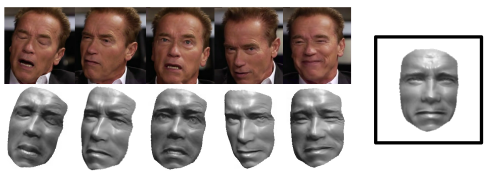
\includegraphics[width=\linewidth]{img/total_moving.png}
  \caption[Example output from Total Moving Face Reconstruction
  method]{Output from~\cite{suwajanakorn2014total}, ``Total Moving
    Face Reconstruction'', on a frame by frame basis, with the average
    of these reconstructions shown on the right.}
  \label{fig:total_moving}
\end{figure}

\paragraph{Reconstruction from video} is perhaps the most generous 3D
face reconstruction problem due to the abundance of data available to
methods. Under this setting, it is quite likely that any given method
is using will exhibit a variety of poses, from which it can base its
reconstruction upon. However, methods working with such data can still
suffer from problems such as occlusion. A high performing method known
as ``Total Moving Face Reconstruction''~\cite{suwajanakorn2014total}
performs 3D face reconstruction from video. We shown an example of
this method on a video in Figure~\ref{fig:total_moving}. In terms of
detail, this method performs very well on a frame by frame
basis. However, we can also see that this method does not
\textit{actually} recover the full 3D geometry, instead, focusing its
attention solely on the frontal region of the face. While doing so,
often cutting off the sides of the face - most notably on the average
of the reconstruction, where a large part the chin is
missing. Finally, while the main goal really is to produce a high
quality reconstruction on a per-frame basis, the method does not
really produce a particularly refined result by combining the temporal
information.



\paragraph{Reconstruction from sets of images} has the potential to
make the problem slightly more challenging than from a full video. One
reason for this is that there is likely less variation in pose
available. However, perhaps more importantly, with video, a 3D mesh
can be provided on a per frame basis, in fact, this is expected from
such a method. The facial expression can be refined over time. In the
case of reconstruction from multiple images though, only a single
model is outputted, taking into account factors from the entire set of
images. At first this may not sound like a big issue, but consider a
set of images where only half the samples are exhibiting large smiles?
Do you produce a smiling or neutral mesh? Of course, many of the
limitations of 3D scanners are shared by methods performing 3D face
reconstruction from sets of images - obtaining a large collection of
images can be just as disruptive as stepping into a 3D scanner.

\begin{wrapfigure}{R}{0.35\textwidth}
  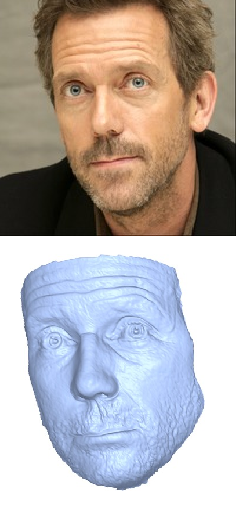
\includegraphics[width=0.3\textwidth,right]{img/unrestricted.png}
  \caption[Example output from Unrestricted Facial Geometry
  Reconstruction method]{An example of a reconstruction from a single,
    frontal image generated by~\cite{sela2017unrestricted}.}
  \label{fig:unrestricted}
\end{wrapfigure}

\paragraph{Reconstruction from a single image} is the undoubtedly
hardest of the three classes of 3D face reconstruction. This is due to
the lack of information from multiple poses, requiring such approaches
to hallucinate or guess a much larger amount of the face. We show in
Figure~\ref{fig:unrestricted} an example result of 3D face
reconstruction performed by~\cite{sela2017unrestricted}, a method
which uses only a single image. This method is often considered state
of the art. Clearly, the level of detail is good, but this is a
completely frontal image with neutral expression. The authors
of~\cite{sela2017unrestricted} state in their section titled
``Limitations'' that images which deviate too much from what the
method was trained on are challenging and result in errors in the
reconstruction process. The authors also state that the method has
difficulty handling cases of occlusion. These statements are supported
by only frontal, non-occluded results being presented in the
paper. Additionally, our own tests of this method have shown
significant failure cases, to the point of the output not even
resembling a face, under even very small pose variations. There is
perhaps an even larger disadvantage of this method. During the detail
extraction precedure of~\cite{sela2017unrestricted}, both pose, scale
and position relative to the original image is discarded, which would
require correction from another method, or manual adjustment to bring
the 3D geometry back into original space of the 2D image.

Given the numerous applications of such a technology and the
significant disadvantages of the preexisting methods, we feel there is
a profound requirement for something more robust to the aforementioned
challenges in this area. To summarise, these challenges include large
pose (in many cases, even small pose), occlusion and expressions. In
this thesis we approach this problem using a single image. We try to
address how we fit into this challenging space in more detail in the
next section.

\section{Where do we fit in?}

There are a number of approaches to 3D face reconstruction. Each
general approach has its own set of advantages and disadvantages. The
aim of this section is to give a brief overview of the general
approaches to this problem. By doing so, we hope to show where and how
our own work fits in, along with why we feel this is important.

% 3D Morphable Models
\paragraph{3D Morphable Models (3DMM)} are perhaps the most popular
approach to estimating facial 3D geometry. These methods regress
parameters for a pre-computed face
model~\cite{jourabloo2016large,huber2016multiresolution,zhu2016face,liu2016joint},
which varies the shape, expression, pose and optionally textural
information. These methods are increasingly using Convolutional Neural
Networks as a means to regress the parameters, and in general, work
very reliably on \textit{normal} faces. However, 3DMM based approaches
gradually perform worse as factors such as pose and expression
increase. We show in Section~\ref{chapter:face:sec:ablation} that our
method has a very uniform and low error over all expressions, with
only a small increase in error on large poses (such as around 80
degrees). Another disadvantage of 3DMM based approaches is that the
3DMM must be generated - this requires finding the dense
correspondence between all vertices of all samples, which also becomes
difficult as pose and expression changes. Finally, since these methods
are modelled, they are unable to directly produce finer details, such
as wrinkles. In an extension to our own work, we show
in Chapter~\ref{chapter:human} (where we perform 3D reconstruction of humans),
that our method is able to directly regress fine details in clothing.


\paragraph{Multiview and Photogrammetry} based methods require
multiple images from many different angles in order to estimate the 3D
geometry of a face (or other
object)~\cite{dou2018multi,dai2018coarse,Piotraschke_2016_CVPR,mayo20093d}. The
primary drawback of such methods is, of course, that multiple images
are not always available, especially under the aforementioned
environmental constraints associated with 3D face
reconstruction. While the final 3D reconstruction from such methods
can be of very high resolution and detailed, finding corresponding
features between each image is both memory and CPU intensive. Our own
method uses only a single RGB image, without any additional depth data
- from this single image, we regress the full 3D facial geometry.

\paragraph{Shape-from-Shading (SfS)} methods attempt to recover the 3D
geometry by analysing the shading and reflectance of a face relative
to a \textit{albedo} (mean) face. Similarly to 3DMM based methods, SfS
methods also tend to rely on a 3D model, inheriting many of the same
problems, such as finding a dense
correspondence~\cite{suwajanakorn2014total,jiang20183d}. Additionally,
many of these methods also require more than one image, which means
SfS methods often also inherit the problems associated with multiview
methods. Finally, more so than other methods, SfS methods struggle
with lighting - in general, there \textit{has} to be shadows, so over
or under illuminated faces may produce poor results when compared to
other methods. Our approach to 3D face reconstruction works under
almost all kinds of lighting, and we show this on a challenging
synthetic dataset.

\paragraph{Depth Estimation} is arguable more popular among problems
such as room reconstruction, however, there are several methods which
attempt to reconstruct the frontal part of the facial 3D geometry
using this technique~\cite{sun2011depth,sun2013depth}. It would be
fair to claim that these methods have declined in popularity. The
biggest flaw of depth estimation based approaches is that only the
visible parts can be reconstructed, unless other methods are employed
afterwards (such as 3DMM, again, inheriting many of the aforementioned
problems). While also working from a single image, our method is able
to hallucinate the non-visible parts of the face, including, to an a
certain extent, those which have been self occluded without having to
handle this cases on an individual basis.

Our method is unique - it doesn't fit into any of these categories. We
present a new approach to 3D face reconstruction which attempts to
account for as many of the challenges in 3D face reconstruction as
possible.

\section{Contributions}

The contributions of this thesis can be summarised as follows:

\begin{itemize}
\item % 3D face reconstruction
  We present a deeply learnt method for 3D face reconstruction, which
  can be trained directly in an end-to-end fashion. Our method
  reconstructs the full 3D facial structure, including parts which are
  occluded. We also show that our method works from just a single
  images without requiring accurate alignment or establishing a dense
  correspondence between all training samples.  This allows us to
  bypass the construction (during training) and fitting (during
  inference) of a 3D Morphable Model (3DMM).  We refer to this method
  as the \textbf{Volumetric Regression Network (VRN)}.

\item We show how a related task of facial landmark localisation can
  be incorporated into our method (also in an end-to-end fashion) to
  improve the reconstruction quality, particularly on faces of large
  pose and expression.

\item We evaluate our method on both constrained and heavily
  unconstrained images from the web, demonstrating that our method
  \textbf{outperforms all prior work} on single image 3D face
  reconstruction by a large margin.

\item We show that our method works on other deformable objects, such
  as in the task of \textbf{human body reconstruction}, and that
  provided high quality training data is available, our method is able
  to both reconstruct difficult human poses and \textbf{fine details
    such as wrinkles} in clothing.

\item We release our code for 3D face reconstruction under the MIT
  license, enabling our method to be used for both commercial and
  personal purposes. In addition, we have provided a free online
  service for automatic generation of 3D reconstructions from an
  uploaded image.
\end{itemize}

\section{Outline}

In \textbf{Chapter~\ref{chapter:background}}, an introduction to the
background material is provided. This includes a brief introduction to
gradient descent based optimisation, an overview of Convolutional
Neural Networks (CNNs) the problems batch normalisation attempts to
solve. This background discussion then moves onto volumetric
representations and algorithms, such as voxelisation, surface
extraction and some of the difficulties associated with volumetric
representations.

\textbf{Chapter~\ref{chapter:literature}} gives an overview of related
literature, starting with face alignment, which is often a
prerequisite to 3D face reconstruction methods. Continuing on, a
discussion of the various existing 3D face reconstruction is
given. The remainder of this chapter gives an overview of human pose
estimation, human body reconstruction and semantic part segmentation.

Our first work, focusing on landmark guided semantic part segmentation
of the human face is described in
\textbf{Chapter~\ref{chapter:seg}}. It is important to mention here
that this thesis does not focus on semantic segmentation, but this
work \textit{heavily} influenced our approach to the problem of 3D
reconstruction, since our method shifts the 3D reconstruction problem
into a volumetric segmentation problem.

\textbf{Chapter~\ref{chapter:face}} is the primary focus of our
thesis. This chapter describes our approach to 3D face reconstruction,
which includes details about the datasets uses, the volumetric
representation and the (small) amount of error it introduces, along
with our approach and network architectures. This chapter also
describes the numerous experiments carried out on the various
datasets, comparisons with other methods, and ablation studies on
pose, expression and influence of parameters used for guidance.

An extension to our work on 3D face reconstruction is described in
\textbf{Chapter~\ref{chapter:human}}, in which we show how our method
can be applied to on another category of deformable objects: the full
human body. We carry out experiments on two datasets, showing that our
approach can handle both difficult poses and finer details.

Finally, we conclude with a reflection and discussion of our work,
what impact it may have had and the numerous areas worthy of attention
as future work, in \textbf{Chapter~\ref{chapter:conclusion}}.

%%% Local Variables:
%%% TeX-master: "../thesis"
%%% End:
